\documentclass[a4paper,12pt]{extarticle}
\usepackage[utf8x]{inputenc}
\usepackage[T1,T2A]{fontenc}
\usepackage[russian]{babel}
\usepackage[hidelinks]{hyperref}
\usepackage{indentfirst}
\usepackage{listings}
\usepackage{color}
\usepackage{here}
\usepackage{array}
\usepackage{multirow}
\usepackage{graphicx}
\usepackage{subcaption} 
\usepackage{mathtools}
\usepackage{listings}

\usepackage{caption}
\renewcommand{\lstlistingname}{Программа} % заголовок листингов кода

\bibliographystyle{ugost2008ls}

\usepackage{listings}
\lstset{ %
extendedchars=\true,
keepspaces=true,
language=C,						% choose the language of the code
basicstyle=\footnotesize,		% the size of the fonts that are used for the code
numbers=left,					% where to put the line-numbers
numberstyle=\footnotesize,		% the size of the fonts that are used for the line-numbers
stepnumber=1,					% the step between two line-numbers. If it is 1 each line will be numbered
numbersep=5pt,					% how far the line-numbers are from the code
backgroundcolor=\color{white},	% choose the background color. You must add \usepackage{color}
showspaces=false				% show spaces adding particular underscores
showstringspaces=false,			% underline spaces within strings
showtabs=false,					% show tabs within strings adding particular underscores
frame=single,           		% adds a frame around the code
tabsize=2,						% sets default tabsize to 2 spaces
captionpos=t,					% sets the caption-position to top
breaklines=true,				% sets automatic line breaking
breakatwhitespace=false,		% sets if automatic breaks should only happen at whitespace
escapeinside={\%*}{*)},			% if you want to add a comment within your code
postbreak=\raisebox{0ex}[0ex][0ex]{\ensuremath{\color{red}\hookrightarrow\space}},
texcl=true,
inputpath=listings,                     % директория с листингами
}

\usepackage[left=2cm,right=2cm,
top=2cm,bottom=2cm,bindingoffset=0cm]{geometry}

%% Нумерация картинок по секциям
\usepackage{chngcntr}
\counterwithin{figure}{section}
\counterwithin{table}{section}

%%Точки нумерации заголовков
\usepackage{titlesec}
\titlelabel{\thetitle.\quad}
\usepackage[dotinlabels]{titletoc}

%% Оформления подписи рисунка
\addto\captionsrussian{\renewcommand{\figurename}{Рисунок}}
\captionsetup[figure]{labelsep = period}

%% Подпись таблицы
%\DeclareCaptionFormat{hfillstart}{\hfill#1#2#3\par}
%\captionsetup[table]{format=hfillstart,labelsep=newline,justification=centering,skip=-10pt,textfont=bf}

%% Путь к каталогу с рисунками
\graphicspath{{fig/}}

%% Внесение titlepage в учёт счётчика страниц
\makeatletter
\renewenvironment{titlepage} {
 \thispagestyle{empty}
}
\makeatother

\DeclarePairedDelimiter\abs{\lvert}{\rvert}%
\DeclarePairedDelimiter\norm{\lVert}{\rVert}%

\usepackage{amsmath}

\begin{document}	% начало документа

% Титульная страница
\begin{titlepage}	% начало титульной страницы

	\begin{center}		% выравнивание по центру

		\large Санкт-Петербургский политехнический университет Петра Великого\\
		\large Институт прикладной математики и механики \\
		\large Кафедра <<Прикладная математика>>\\[6cm]
		% название института, затем отступ 6см
		
		%\huge Математическая статистика\\[0.5cm] % название работы, затем отступ 0,5см
		\huge Методы оптимизации\\[0.5cm] % название работы, затем отступ 0,5см
		%\large \textbf{Отчет по лабораторной работе №4}\\[5.1cm]
		\large \textbf{Отчет по лабораторной работе \\``Решение задач одномерной минимизации ``}\\[5.1cm]
		%\\[5cm]

	\end{center}


	\begin{flushright} % выравнивание по правому краю
		\begin{minipage}{0.25\textwidth} % врезка в половину ширины текста
			\begin{flushleft} % выровнять её содержимое по левому краю

				\large\textbf{Работу выполнил:}\\
				\large Колесник В.Н.\\
				\large {Группа:} 3630102/70201\\
				
				\large \textbf{Преподаватель:}\\
				\large к.ф.-м.н., доцент\\
				%\large Баженов Александр Николаевич
				\large Родионова Елена Александровна

			\end{flushleft}
		\end{minipage}
	\end{flushright}
	
	\vfill % заполнить всё доступное ниже пространство

	\begin{center}
	\large Санкт-Петербург\\
	\large \the\year % вывести дату
	\end{center} % закончить выравнивание по центру

\end{titlepage} % конец титульной страницы

\vfill % заполнить всё доступное ниже пространство


% Содержание
\renewcommand\contentsname{\centerline{Содержание}}
\tableofcontents
\newpage

\section{Постановка задачи}
Дана функция:
\begin{equation}
f(x) = x^2 - x + 1
\end{equation}
Дан интервал:
\begin{equation}
[a, b] = [-1, 3]
\end{equation}
Задана точность:
\begin{equation}
\varepsilon_1 = 0.1; \varepsilon_2 = 0.01; \varepsilon_3 = 0.001
\end{equation}
Необходимо найти минимум функции на заданном интервале методами одномерной минимизации (метод дихотомии и метод Фибоначчи) с заданной точностью.\\
\\
Кроме того необходимо посчитать, сколько раз за время работы метода была вычислена исходная функция, и вывести формулу для подсчета ожидаемого количества обращений к исходной функции в зависимости от заданной точности.

\section{Исследование применимости методов}
Для работы обоих методов необходимо выполнение 2 условий:
\begin{itemize}
\item Функция цели должна быть унимодальной на заданном отрезке.
\item Отрезок должен быть конечной длины.
\end{itemize}
Очевидно, что 2 пункт выполнен, а для демонстрации выполнения 1 пункта приводится график функции на заданном отрезке. Красная линия соответствует функции цели, синяя и черная прямые задают левую и правую границы соответственно. Из графика видно, что на заданном отрезке функция достигает минимума в единственной точке, которая не является границей. Это и означает, что функция унимодальна.

\begin{figure}[!htb]
    \centering
    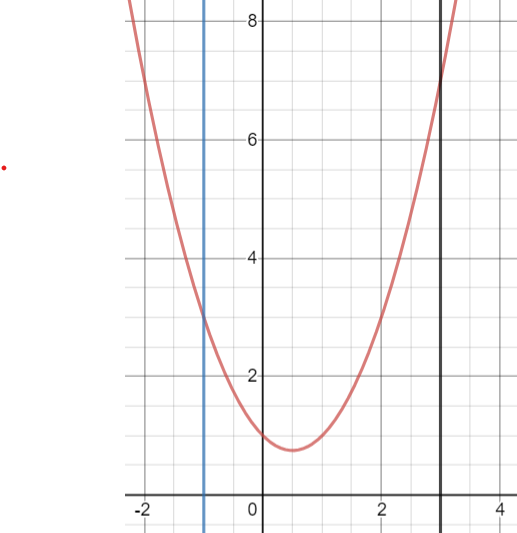
\includegraphics[width=0.25\textwidth]{plot}
    \caption{График функции}
    \label{fig:proof}
\end{figure}

\section{Описание алгоритмов}
\subsection{Метод дихотомии}
\subsubsection{Алгоритм}
Зададим $\delta=0.1\%(b-a)$. Если $2\delta\geq\varepsilon$, то уменьшаем $\delta$ (например, делением на 2), пока в неравенстве знак не поменяется на <.\\
Пусть $a_l = a, b_r=b$.
\begin{enumerate}
  \item $c := \frac{a_l+b_r}{2}$\\
  $x_l := c - \delta$\\
  $x_r := c + \delta$
  \item Вычислим:\\
  $y_l := f(x_l)$\\
  $y_r := f(x_r)$
  \item Если $y_l < y_r$, то $b_r = x_r$.\\
  Иначе $a_l := x_l$
  \item Если $b_r - a_l < \varepsilon$, то закончим алгоритм с ответом $(a_l, b_r)$.\\
  Иначе вернемся к шагу 1. 
\end{enumerate}

\subsubsection{Комментарии к алгоритму}
Выполнение условия $2\delta<\varepsilon$ гарантирует, что 2 точки в окрестности центра всегда буду в текущем отрезке; за границы $a_l$ и $b_r$ они не выйдут.

\subsubsection{Ожидаемое количество вычислений функции}
Длина следующего отрезка равна:\\
\begin{equation}
d_{k+1}=\frac{d_k}{2}+\delta
\end{equation}
Получаем из рекуррентного соотношения:\\
\begin{equation}
d_{n}=\frac{d_0}{2^n}+\delta\sum_{i=0}^{n-1} \frac{1}{2^i}
\end{equation}
Учитывая неравенство для заданной точности, запишем следующее (зададим более сильное условие):\\
\begin{equation}
d_{n}=\frac{d_0}{2^n}+\delta\sum_{i=0}^{n-1} \frac{1}{2^i}<\frac{d_0}{2^n}+2\delta<\varepsilon
\end{equation}
Откуда:\\
\begin{equation}\label{dich}
2^n>\frac{d_0}{\varepsilon-2\delta}
\end{equation}
Справа положительная величина, поэтому можно найти $n$ для заданного отрезка и заданной точности, если известно $\delta$.\\
На каждом шаге значение функции вычисляется 2 раза, поэтому общее число обращений к целевой функции будет не больше $2n$.

\subsection{Метод Фибоначчи}
\subsubsection{Алгоритм}
Пусть $n$ - наименьшее натуральное число такое, что $F_n > \frac{b-a}{\varepsilon}$, где $F_n$ - $n$-ое число Фибоначчи ($F_0=1; F_1=1; F_{i+1}=F_i+F_{i-1}$).\\
Сгенерирурем $n+1$ чисел Фибоначчи (до $F_n$ включительно).\\
Пусть $a_l = a, b_r=b$.
\begin{enumerate}
	\item $k:=1$\\
	Вычислим:\\
	$\lambda:=a_l+\frac{F_{n-k-1}}{F_{n-k+1}}(b_r-a_l)$\\
	$\mu:=a_l+\frac{F_{n-k}}{F_{n-k+1}}(b_r-a_l)$\\
	$y_l := f(\lambda)$\\
	$y_r := f(\mu)$
	\item $k:=k+1$
	\item Если $y_l < y_r$, то перейдем к шагу 4.\\
	Иначе перейдем к шагу 5.
	\item $b_r :=\mu$\\
	$\mu:=\lambda$\\
	$y_r:=y_l$\\
	$\lambda:=a_l+\frac{F_{n-k-1}}{F_{n-k+1}}(b_r-a_l)$\\
	$y_l := f(\lambda)$\\
	Перейдем к шагу 6.
	\item $a_l:=\lambda$\\
	$\lambda:=\mu$\\
	$y_l:=y_r$\\
	$\mu:=a_l+\frac{F_{n-k}}{F_{n-k+1}}(b_r-a_l)$\\
	$y_r := f(\mu)$\\
	Перейдем к шагу 6.
	\item Если $k=n-2$, перейдем на следующий шаг.\\
	Иначе вернемся к шагу 2.
	\item Если $y_l < y_r$, то перейдем к шагу 7.\\
	Иначе перейдем к шагу 8.
	\item $b_r :=\mu$\\
	$\mu:=\lambda$\\
	$y_r:=y_l$\\
	$c:=\mu$\\
	Перейдем к шагу 10.
	\item $a_l:=\lambda$\\
	$\lambda:=\mu$\\
	$y_l:=y_r$\\
	$c:=\lambda$\\
	Перейдем к шагу 10.
	\item Зададим $\delta=0.1\%(b_r-a_l)$. Если $\delta + c - a_l\geq\varepsilon$, то уменьшаем $\delta$ (например, делением на 2), пока в неравенстве знак не поменяется на <.
	\item $\mu:=c+\delta$\\
	$y_r:=f(\mu)$
	\item Если $y_l < y_r$, то $b_r :=\mu$.\\
	Иначе $a_l:=c$.\\
	Закончим алгоритм с ответом $(a_l, b_r)$
\end{enumerate}

\subsubsection{Комментарии к алгоритму}
Несложно строго показать, что при $k=n-1$ $\lambda$ и $\mu$ окажутся равными и будут находиться в середине текущего отрезка. В таком случае не удастся выбрбать нужную половину отрезка. Поэтому в данном алгоритме при $k=n-1$ берется очень близкая к центру текущего отрезка точка, в которой вычисляется значение функции, и по ней определяется финальный отрезок.\\
На шаге 11 можно отсутпить не вправо от центра, а влево:\\
$\lambda:=c-\delta$\\
$y_l:=f(\lambda)$

\subsubsection{Ожидаемое количество вычислений функции}
Известно, что длина следующего отрезка не зависит от выбора $\mu$ или $\lambda$ и равна:\\
\begin{equation}
d_{k+1}=\frac{F_{n-k}}{F_{n-k+1}}(b_k-a_k)=\frac{F_{n-k}}{F_{n-k+1}}d_k
\end{equation}
Получаем из рекуррентного соотношения:\\
\begin{equation}
d_{n}=\prod_{k=1}^{n-1}\frac{F_{n-k}}{F_{n-k+1}}d_0=\frac{F_{1}}{F_{n}}d_0=\frac{b-a}{F_{n}}
\end{equation}
Неравенство для заданной точности:\\
\begin{equation}
d_{n}=\frac{b-a}{F_{n}}<\varepsilon
\end{equation}
Откуда:\\
\begin{equation}\label{fib}
F_n>\frac{b-a}{\varepsilon}
\end{equation}
Так можно найти $n$ для заданного отрезка и заданной точности.\\
На 1 шаге $k=1$ значение целевой функции вычисляется 2 раза, на всех остальных - 1 раз, $k$ пробегает значения от 1 до n-1. Таким образом, значение функции вычисляется n раз.

\section{Результаты решения}
Для данной задачи ожидаемое количество вычислений целевой функции в соответствии с (\ref{dich}) и (\ref{fib}) представлено в таблицах.

\begin{table}[h]
	\centering
		\begin{tabular} {|c|c|c|c|c|}
			\hline
			$\varepsilon$ & $\frac{b-a}{\varepsilon}$ & $\frac{b-a}{\varepsilon - 2\delta}$ & $n$ для метода дихотомии & $n$ для метода Фибоначчи \\ \hline
			0.1 & 40 & 43.5 &6 & 9\\ \hline
			0.01 & 400 & 2000 & 12 & 14\\ \hline
			0.001 & 4000 & 8000 & 14 &  18\\ \hline
		\end{tabular}
		\caption{Подсчет $n$}
	\end{table}
		\newpage

\begin{table}[h]
	\centering
		\begin{tabular} {|c|m{3 cm}|m{3 cm}|m{3 cm}|m{3 cm}|}
			\hline
			$\varepsilon$ & Теор. ожидание для метода дихотомии & Реальное количество для метода дихотомии &Теор. ожидание для метода Фибоначчи & Реальное количество для метода Фибоначчи  \\ \hline
			0.1 & 12 & 12 & 9 & 9\\ \hline
			0.01 & 24 & 22 & 14 & 14\\ \hline
			0.001 & 28 & 26 & 18 &  18\\ \hline
		\end{tabular}
		\caption{Ожидаемые и реальные количества вызовов целевой функции}
	\end{table}

Из таблицы видно, что для метода Фибоначчи теоретическая оценка количества обращений к целевой функции оказалась точной - она совпала во всех 3 случаях. Для метода дихотомии в 2 случаях оценка оказалась выше - ожидалось на 1 итерацию больше.\\
Кроме того, из таблицы видно, что для метода Фибоначчи вычислять целевую функцию надо реже, чем в методе дихотомии.

\section{Обоснование достоверности полученного результата}
Аналитически и графически можно проверить, что минимум функции на заданном отрезке достигается в $x=0.5$.\\
\begin{figure}[!htb]
    \centering
    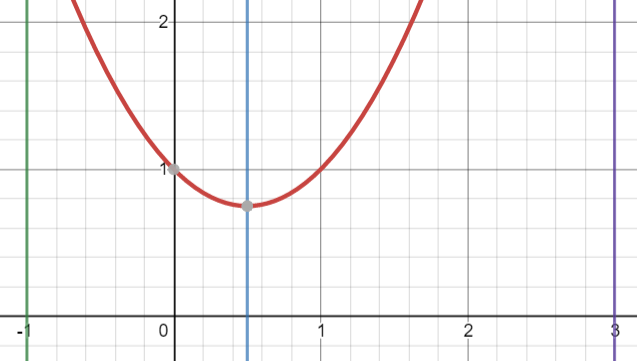
\includegraphics[width=0.25\textwidth]{plot2}
    \caption{График функции}
    \label{fig:proof}
\end{figure}\\
Представим в виде таблицы результаты работы обоих методов.\\
\begin{table}[h]
	\centering
		\begin{tabular} {|c|m{3 cm}|m{3 cm}|m{3 cm}|m{3 cm}|}
			\hline
			$\varepsilon$ & Интервал методом дихотомии & Длина интервала методом дихотомии & Интервал методом Фибоначчи & Длина интервала методом дихотомии \\ \hline
			0.1 & (0.43, 0.50) & 0.07 & (0.45, 0.52)& 0.07\\ \hline
			0.01 & (0.495, 0.505) & 0.009 & (0.495, 0.502) & 0.007\\ \hline
			0.001 & (0.4993, 0.5003) & 0.0009 & (0.4992, 0.5001) &  0.0009\\ \hline
		\end{tabular}
		\caption{Решения}
	\end{table}\\
По таблице видно, что истинный минимум попадает во все полученные обоими методами интервалы неопределенности для всех 3 заданных точностей. В некоторых случаях метод Фибоначчи давал более точное решение, чем метод дихотомии.


\end{document}
